\subsection{哪里最好躲：藏得住，也要走得到}
\label{sec:res-spot}
图~\ref{fig:spot}a 把“开局被随机分到某个藏身点的老鼠活了多久”画在地图上。需要说明，这里按老鼠\textbf{开局被分到的目的地}分组：老鼠在藏身点被发现、逃跑之后会换地方，所以它的存活时间并不全是在这个点上挣到的。

最出乎意料的是图~\ref{fig:spot}b：被分到灌木丛和被分到夹缝的老鼠，平均存活分别是 9.3 分钟和 9.6 分钟，同一局内配对的差只有 0.3 分钟（95\% 区间 [$-0.19$, 0.77]），没有显著差别。可是在第~\ref{sec:res-campus} 节里，“只躲夹缝”比“只躲灌木”多活 4.7 分钟。两个实验的差别在于选点方式：第~\ref{sec:res-campus} 节的老鼠是\textbf{就近}选点。在 A–G 楼一带，夹缝紧贴每栋楼的外墙，从集合点出发走几十米就有；成片的灌木则多在场地边缘，离集合点 100 m 以上（图~\ref{fig:env}a）。就近选灌木的老鼠，要么只能找到零星的小块灌木，要么要穿过大片空地才能藏好，路上就被看见了。所以一个藏身点好不好取决于两件事：藏得住，以及走得到。夹缝两样都占，这与实战中“鼠王躲在夹缝里，一直到最后都没有被抓到”的经验一致（RQ2）。图~\ref{fig:spot}c 中，存活时间随藏身点到集合点的距离没有明显趋势，各组区间都很宽。

\begin{figure}[htbp]
  \centering
  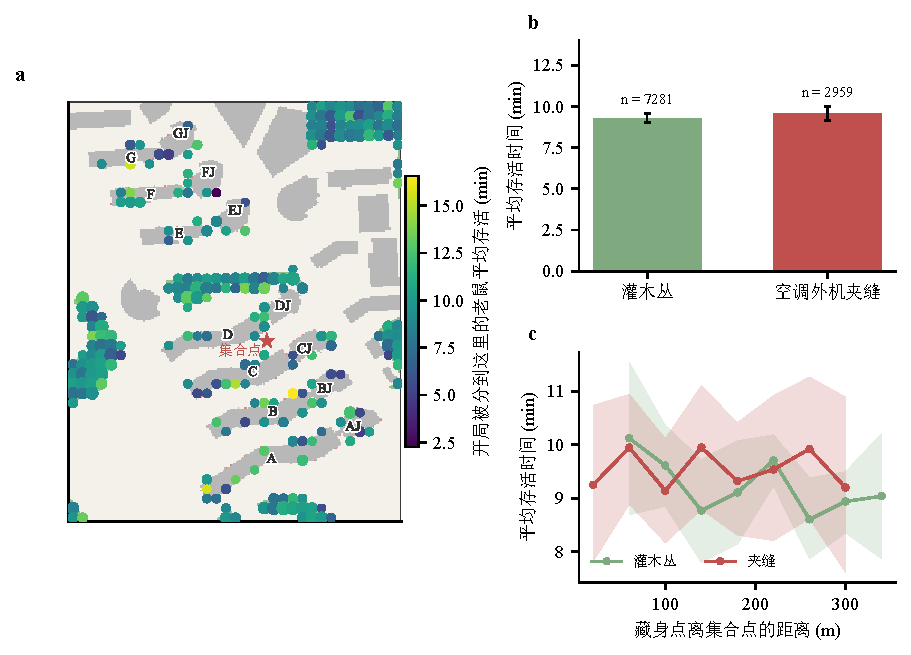
\includegraphics[width=\textwidth]{fig4_where_to_hide.pdf}
  \caption{\figlead{一旦被分到藏身点，灌木和夹缝一样安全；夹缝的优势在于离每个人都近。}
  \textbf{a}，每只老鼠开局被随机分到一个藏身点。圆点是 12 m 格内老鼠的平均存活时间（只画至少 15 只老鼠的格子），点越大样本越多；红星为集合点。
  \textbf{b}，按开局目的地的类型汇总，误差棒为按局自举的 95\% 区间。
  \textbf{c}，存活时间随藏身点到集合点距离的变化（40 m 一组，只画至少 100 只老鼠的组），阴影为 95\% 区间。共 2 × 256 局、10240 只老鼠（灌木 7281 只，夹缝 2959 只），每局 30 分钟。}
  \label{fig:spot}
\end{figure}

\subsection{上下两轮之间：会从跑转向躲，也会从躲转向跑}
\label{sec:res-rounds}
先看收益（图~\ref{fig:rounds}a）。不管第一轮有多少人躲，躲者都比跑者多活 4.5–5.5 分钟：躲者的平均存活在 9.3–10.2 分钟之间，跑者在 4.7–5.0 分钟之间。也就是说，在这个模型里“躲”是严格占优的策略，复制者动态\cite{taylor1978}唯一的稳定点是“全员都躲”。两条曲线随 $x$ 的变化都很小：躲的人越多，躲者自己略差一点（10.2 → 9.3 分钟，可能是近处的好位置被占满了），跑者基本不变（4.7–5.0 分钟）。所以每只老鼠的收益主要取决于自己怎么做，几乎不取决于别人怎么做。

再看个体模仿（图~\ref{fig:rounds}b，$K=1$ 分钟）。看到别人的结果后，第二轮确实会有人从跑转向躲：第一轮躲的比例为 0.25、0.5、0.75 时，分别有 15\%、29\%、42\% 的跑者改成躲。反方向的转化也确实存在，而且不少：同样三种情况下，分别有 34\%、24\%、12\% 的躲者改成跑。原因是单局结果的随机性很大：全员都躲时，约五分之一的老鼠能撑满 30 分钟，但也有不少人一藏好就被路过的猫看见了；一个运气差的躲者看到一个运气好的跑者，就可能改成跑。两个方向相互抵消后，第二轮躲的比例只比第一轮高 0.01–0.02（例如 0.25 → 0.27）。把 $K$ 换成 3 分钟，结果几乎不变，因为单局之间的存活差距通常远大于 3 分钟。

这对实际游戏的含义是：只看一局、只看身边一个人，“躲更好”这个结论很难传开；如果第一轮结束后有人公布\textbf{平均}结果（相当于看很多人的结果），转化会快得多。

\begin{figure}[htbp]
  \centering
  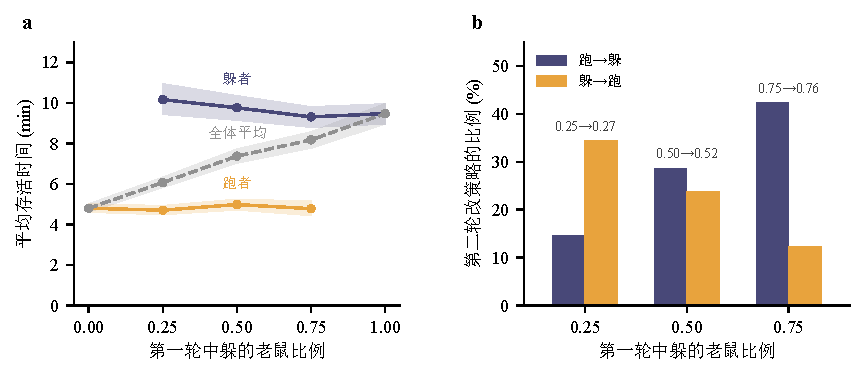
\includegraphics[width=\textwidth]{fig6_between_rounds.pdf}
  \caption{\figlead{躲在任何比例下都比跑好，但只看身边一个人的结果时，两个方向的转化都会发生，躲的比例上升得很慢。}
  \textbf{a}，第一轮中躲的比例为 $x$ 时，躲者、跑者和全体老鼠的平均存活时间（30 分钟一轮），阴影为按局自举的 95\% 区间，每个 $x$ 256 局。
  \textbf{b}，第一轮结束后每只老鼠随机看同局一个同伴，按费米模仿规则（$K=1$ 分钟）决定是否改用同伴的策略。柱是两个方向的转化比例，柱顶数字是第一轮和第二轮躲的比例。}
  \label{fig:rounds}
\end{figure}
